% Draft (2026-11-07). \tbd{} marks numbers from the preregistered E1 test run.
\section{What natural audit failures are made of}
\label{sec:natural}

The randomised experiment isolates the information limit on constructed units. We ask how much of an ordinary audit
benchmark is subject to that limit. We use 150 programs written by two generator models for HumanEval+ and MBPP+
problems. Each program passes its visible tests but fails the hidden suite and is paired with a test-passing control
\citep{liu2023evalplus}.

\paragraph{Most hidden-test failures are not determined by the task.} Two models classify each program's first failing
input, blind to which output is the benchmark's (order randomised by evidence). The categories are: the input is
outside the task's domain, only the reference's output is acceptable (\textsc{determined}), both are
(\textsc{open}), only the program's is (\textsc{at odds}), or neither. Identical evidence is pooled so that it cannot
receive two labels. Of the 150 failures, 34 are \textsc{determined}, 26 \textsc{open}, 37 \textsc{at odds},
21 out of domain and 32 disputed (Cohen's $\kappa=0.78$ on the 43 development items). Only on 34 of the 150 (23\%) do
both classifiers agree that the task's words single out the value the hidden suite expects; on 63 they agree that
the words leave it open or point the other way.

\paragraph{Other solutions mostly side with the ``defective'' program.} A behavioural check avoids classifier
judgement. For each failure, two generators wrote twelve solutions from the task alone; we run the 1{,}710
of the 1{,}800 that pass the visible tests on the same first failing input. They return the defective program's
result 1{,}080 times and the reference's 559 times (71 neither); for 93 failures most solutions side with the
defective program, for 46 with the reference. The solutions come from the same two generators that wrote the failing
programs, so this is partly a model agreeing with itself; still, on the inputs that define these programs as
defective, the benchmark's expected value is the minority reading among solutions written from the task. The
behaviour also checks the classification (Figure~\ref{fig:natural}b): where the classifiers judge that only the
program's output fits the words (\textsc{at odds}), 90\% of independent solutions return it; where they judge the
reference's value determined, solutions split almost evenly, which is consistent with defects the generators commonly
share.

\begin{figure}[t]
\centering
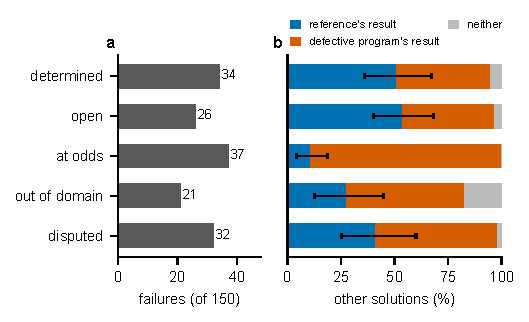
\includegraphics[width=\columnwidth]{fig_natural.pdf}
\caption{Natural hidden-test failures (150 programs that pass their visible tests). (a) Class of the first failing
input, as two classifiers judge it from the task's words and visible tests, with identical evidence pooled. (b) What
independent solutions written from the task alone (and passing the visible tests) return on that input, by class;
the interval is an item-level bootstrap for the share returning the reference's result.}
\label{fig:natural}
\end{figure}

\paragraph{What auditors verify.} With the original task text, four readings per program and two auditors, verified
diagnosis on the held-out failures is \NOneVdDetermined\% on \textsc{determined} failures and \NOneVdOpen\% on
\textsc{open} ones. The registered contrast (H6) is \NOneHSix{} points [\NOneHSixLo, \NOneHSixHi] and is not
supported: on these failures the class of the first failing input does not predict whether an auditor verifies a
defect (the development estimate, from 13 items, was 50 points). The witnesses tell a more specific story. Of the
\NOneBridgeItems{} held-out programs with a verified diagnosis, \NOneBridgeDetermined{} have at least one witness that
both classifiers label \textsc{determined}: an auditor that verifies a defect in an \textsc{open} failure usually does
so through a different input, on which the words do decide. Hidden-test recall on such a benchmark therefore mixes
two things: on behaviour the words determine it measures the auditor, and elsewhere it measures at best agreement
with a convention the task does not state. The classification concerns the first failing input only, so a program
may also have determined defects elsewhere.

\paragraph{Clarifying the missing requirement.} For the 13 failures that remain \textsc{open} after reclassification
and whose added sentences pass a neutrality recheck, we appended the missing requirement as one sentence, a
length-matched placebo, or a pointer naming the input class without resolving it. The \NOneItems{} held-out items
(\NOneProblems{} problems) provide a small replication of Section~\ref{sec:e6}: the clause raises verified
diagnosis by \NOneHOne{} points [\NOneHOneLo, \NOneHOneHi] over the placebo (H1) and by \NOneHFive{} points
[\NOneHFiveLo, \NOneHFiveHi] over the pointer (H5), and the placebo does nothing (H4). Whether the clause also
raises flags on correct programs could not be settled at this size (H2: $-$5.6 points [$-$33.3, 22.2]).
